%----------------------------------------------------------------------------------------
%    PACKAGES AND THEMES
%----------------------------------------------------------------------------------------

\documentclass[aspectratio=169,xcolor=dvipsnames]{beamer}
\usetheme{SimpleDarkBlue}

\usepackage{hyperref}
\usepackage{graphicx} % Allows including images
\usepackage{booktabs} % Allows the use of \toprule, \midrule and \bottomrule in tables
\usepackage{biblatex}
\addbibresource{mlops.bib}
\graphicspath{{./images/}}
%----------------------------------------------------------------------------------------
%    TITLE PAGE
%----------------------------------------------------------------------------------------

\title{Brute-forcing Monte Carlo Simulation}

\author{Radu Briciu}

\institute
{
	BSc Finance (Hons) \\ 
	University of Westminster \\
	\vspace*{1em}
	City, University of London \\
	Faculty of Finance
}
\date{\today} % Date, can be changed to a custom date

%----------------------------------------------------------------------------------------
%    PRESENTATION SLIDES
%----------------------------------------------------------------------------------------

\begin{document}
	
	\begin{frame}
		% Print the title page as the first slide
		\titlepage
	\end{frame}
	
	\begin{frame}{Overview}
		In this session we explore a proposed method for estimating nonlinear stochastic functions in the context of path dependent financial derivatives
		\tableofcontents
	\end{frame}
	
	%------------------------------------------------
	\section{Financial Derivatives}
	%------------------------------------------------
	
	\begin{frame}{Financial Derivatives}
		What are financial derivatives?
		\begin{figure}[h]
			\centering
			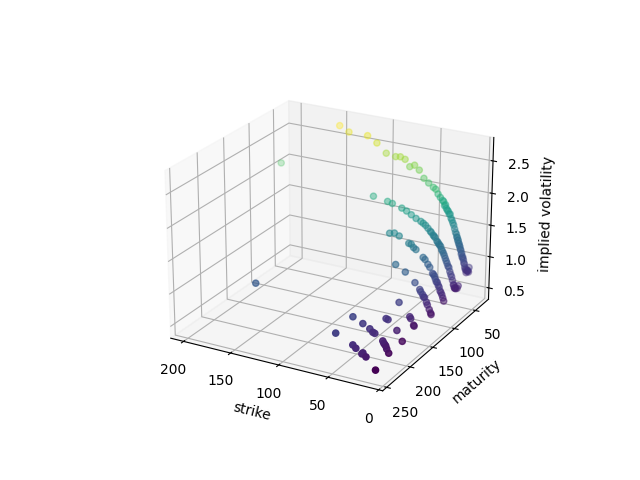
\includegraphics[width=0.5\textwidth]{vix.png}
		\end{figure}
	\end{frame}
	
	\begin{frame}{Financial Derivatives}
		We can begin thinking about the problem by advancing on the illustrious concept of the Myron Black and Fischer Scholes pricing model for plain European call options.
		\begin{align}
			C_{t} &= S_{t} N(d_{1}) - K e^{-r(T-t)} N(d_{2}) \\
		\end{align} where
		\begin{align}
			d_{1} &= \frac{\ln(\frac{S}{K}) + (r+\frac{\sigma^{2}}{2})(T-t)}{\sigma\sqrt{T-t}} \; \; \text{and} \\
			d_{2} &= d_{1} - \sigma \sqrt{T-t}
		\end{align}
	\end{frame}
	
	\begin{frame}{Financial Derivatives}
		Problems with the classical Black-Scholes model (as presented):
		\begin{itemize}
			\item{Constant volatility}
			\item{Arbitrage free}
			\item{Instantaneous returns}
			\item{No dividends}
			\item{Cannot price complex financial derivatives}
		\end{itemize}
	\end{frame}
	
	%------------------------------------------------
	\section{Remedy}
	%------------------------------------------------
	
	\begin{frame}{The Heston (1993) Model}
		\begin{itemize}
			\item Geometric Brownian Motion
			\item Arbitrary correlation between asset volatility and return
		\end{itemize}
		\begin{align}
			dS_t &= \left( r - \frac{v_t}{2} \right) dt + \sqrt{v_t} \left( \rho dW_t + \sqrt{1 - \rho^2} dB_t \right) \label{eq:hdXt} \\
			dv_t &= \kappa (\theta - v_t) dt + \eta \sqrt{v_t} dW_t \hspace{1.8cm} \label{eq:hdvt}
		\end{align}
		\begin{enumerate}
			\item $v_0$ represents the initial variance,
			\item $\theta$ is the long-run variance,
			\item $\rho$ is the correlation between the log-price process and its volatility,
			\item $\kappa$ is the mean reversion of the variance to $\theta$,
			\item $\eta$ is the volatility of the variance process, and 
			\item $B_{t}$, $W_{t}$ are continuous random walks.
		\end{enumerate}
	\end{frame}
	
	\begin{frame}{Applications}
	Calibration of the Heston (1993) model permits usage of more sophisticated pricing algorithms in determining a correct asset price. We are able to leverage path-dependent dynamics of the underlying price to create more sophisticated financial derivative products. One such example is the \textit{Asian} option:
		\begin{align}
			C^{\text{Asian}}_t &= e^{-r(T-t)} \times \frac{1}{m} \sum_{i=1}^{m} (S_{T}^{\text{avg}} - K)^{+} \\
		\end{align}
		where $S_{T}^{\text{avg}}$ is the average price of the underlying spot price
	\end{frame}
	
	\begin{frame}{References}
		\nocite{*}
		\printbibliography
	\end{frame}
	
	%------------------------------------------------
	
	\begin{frame}
		\Huge{\centerline{\textbf{The End}}}
	\end{frame}
	
	%----------------------------------------------------------------------------------------
	
\end{document}